\documentclass[landscape,a0paper,fontscale=0.292]{baposter}

\usepackage[vlined]{algorithm2e}
\usepackage{times}
\usepackage{calc}
\usepackage{url}
\usepackage{graphicx}
\usepackage{amsmath}
\usepackage{amssymb}
\usepackage{relsize}
\usepackage{multirow}
\usepackage{booktabs}

\usepackage{graphicx}
\usepackage{multicol}
\usepackage[T1]{fontenc}
\usepackage{ae}
\usepackage{enumitem}

\usepackage{colortbl}
\usepackage{xcolor}
\graphicspath{{images/}}

\setlist[itemize]{leftmargin=*,nosep}
 \setlength{\columnsep}{0.7em}
 \setlength{\columnseprule}{0mm}


 \definecolor{cuhksz}{RGB}{110, 35, 103}

% %%%%%%%%%%%%%%%%%%%%%%%%%%%%%%%%%%%%%%%%%%%%%%%%%%%%%%%%%%%%%%%%%%%%%%%%%%%%%%%%
% % Save space in lists. Use this after the opening of the list
% %%%%%%%%%%%%%%%%%%%%%%%%%%%%%%%%%%%%%%%%%%%%%%%%%%%%%%%%%%%%%%%%%%%%%%%%%%%%%%%%
 \newcommand{\compresslist}{%
 \setlength{\itemsep}{0pt}%
 \setlength{\parskip}{0pt}%
 \setlength{\parsep}{0pt}%
 }
\renewcommand{\rmdefault}{ptm} % Arial
\renewcommand{\sfdefault}{ptm} % Arial

%%%%%%%%%%%%%%%%%%%%%%%%%%%%%%%%%%%%%%%%%%%%%%%%%%%%%%%%%%%%%%%%%%%%%%%%%%%%%
%% Begin of Document
%%%%%%%%%%%%%%%%%%%%%%%%%%%%%%%%%%%%%%%%%%%%%%%%%%%%%%%%%%%%%%%%%%%%%%%%%%%%%
\begin{document}
%%%%%%%%%%%%%%%%%%%%%%%%%%%%%%%%%%%%%%%%%%%%%%%%%%%%%%%%%%%%%%%%%%%%%%%%%%%%%
%% Here starts the poster
%%---------------------------------------------------------------------------
%% Format it to your taste with the options
%%%%%%%%%%%%%%%%%%%%%%%%%%%%%%%%%%%%%%%%%%%%%%%%%%%%%%%%%%%%%%%%%%%%%%%%%%%%%
\begin{poster}{
 % Show grid to help with alignment
 grid=false,
 columns=5,
 % Column spacing
 colspacing=0.7em,
 % Color style
 headerColorOne=cuhksz,
 borderColor=cuhksz,
 % Format of textbox
 textborder=faded,
 % Format of text header
 headerborder=open,
 headershape=roundedright,
 headershade=plain,
 background=none,
 bgColorOne=white,
 headerheight=0.12\textheight}
 % Eye Catcher
 {
      \includegraphics[width=0.1\linewidth]{CUSZ}
 }
 % Title
 {\sc\huge\bf HighEr-Resolution Network for Image Demosaicing and Enhancing}
 % Authors
 {\vspace{0.3em} Kangfu Mei$^1$, Juncheng Li$^2$, Jiajie Zhang$^3$, Haoyu Wu$^1$, Jie Li$^1$, Rui Huang$^{14}$ \\[0.2em]
 {\normalsize $^1$ The Chinese University of Hong Kong, Shenzhen , $^2$ East China Normal University\\ $^3$Kuaishou Technology, $^4$Shenzhen Institute of Artificial Intelligence and Robotics for Society \\[0.2em] }}
 % University logo
 {
    \begin{tabular}{r}
        \includegraphics[width=0.15\linewidth]{iccv19}
    \end{tabular}
 }

%%%%%%%%%%%%%%%%%%%%%%%%%%%%%%%%%%%%%%%%%%%%%%%%%%%%%%%%%%%%%%%%%%%%%%%%%%%%%%
%%% Now define the boxes that make up the poster
%%%---------------------------------------------------------------------------
%%% Each box has a name and can be placed absolutely or relatively.
%%% The only inconvenience is that you can only specify a relative position 
%%% towards an already declared box. So if you have a box attached to the 
%%% bottom, one to the top and a third one which should be inbetween, you 
%%% have to specify the top and bottom boxes before you specify the middle 
%%% box.
%%%%%%%%%%%%%%%%%%%%%%%%%%%%%%%%%%%%%%%%%%%%%%%%%%%%%%%%%%%%%%%%%%%%%%%%%%%%%%

%%%%%%%%%%%%%%%%%%%%%%%%%%%%%%%%%%%%%%%%%%%%%%%%%%%%%%%%%%%%%%%%%%%%%%%%%%%%%%
\headerbox{\bf \color{white} Problem and Contribution}{name=contribution,column=0,row=0,span=2}{
    \textbf{\color{red}Goal:} Learn to restore RGB images generated by DSLR from unprocessed-RAW images generated by smartphones (AIM2019 RAW to RGB Challenge).
    \begin{center}
        \vspace{-0.8em}
        \centering\includegraphics[width=0.8\linewidth]{images/tasks}
    \end{center}

    \vspace{-0.8em}
    \textbf{\color{red}Key Contributions:}
    \begin{itemize}
        \item We propose a HighEr-Resolution Network (HERN), which can fully learning local and global information in high-resolution image patches.
        \item We propose a progressive training method to solve the instability issue and accelerate model convergence.
        \item Our HERN won second place on track 1 (Fidelity) and won first place on track 2 (Perceptual) in the AIM2019 RAW to RGB Mapping Challenge.
    \end{itemize}  
}

%%%%%%%%%%%%%%%%%%%%%%%%%%%%%%%%%%%%%%%%%%%%%%%%%%%%%%%%%%%%%%%%%%%%%%%%%%%%%%
\headerbox{\bf\color{white} Experiments \& Results}{name=results,column=2,row=0,span=3}{
    \begin{minipage}[t]{0.48\textwidth}
        \textbf{Provided Datasets for Training:}
        The provided datasets ZRR for traning contains 89000 train image patches of size 224x224 pixels.
        Some samples is visualized at below:
        \vspace{-0.2em}
        \begin{center}
            \includegraphics[width=\textwidth]{images/datasets}
        \end{center}
    \end{minipage}
    \hfill
    \begin{minipage}[t]{0.48\textwidth}
        \textbf{AIM2019 RAW to RGB Mapping Challenge Results} 
        \vspace{-0.2em}
        \begin{center}
            \includegraphics[width=0.72\textwidth]{images/ranks}
        \end{center}
    \end{minipage}

    \vspace{0.4em}

    \begin{minipage}[t]{0.48\textwidth}
        \textbf{GPU Memory Usage in Differen Resolution:}
        The GPU memory usage will increases when the resolution of image patches increase.
        Therefore, it is unrealistic to train state-of-the-art methods on one GPU card with image patches of 224 * 224 pixels
        \vspace{-0.5em}
        \begin{center}
            \includegraphics[width=0.8\textwidth]{images/gpu_memories}
        \end{center}
    \end{minipage}
    \hfill
    \begin{minipage}[t]{0.465\textwidth}
    \textbf{Artifacts by Resolution Un-Consistent:} 
    (a) shows the local artifacts in the wall area, which is generated by the model without the Pyramid Full-Image Encoder.
    (b) shows clear results in the wall area, which is generated by the model with the Pyramid Full-Image Encoder.
    The used image is full-resolution (2052*1509 px) while the network is trained in resolution of 224*224 px.
        \begin{center}
            \vspace{-0.5em}
            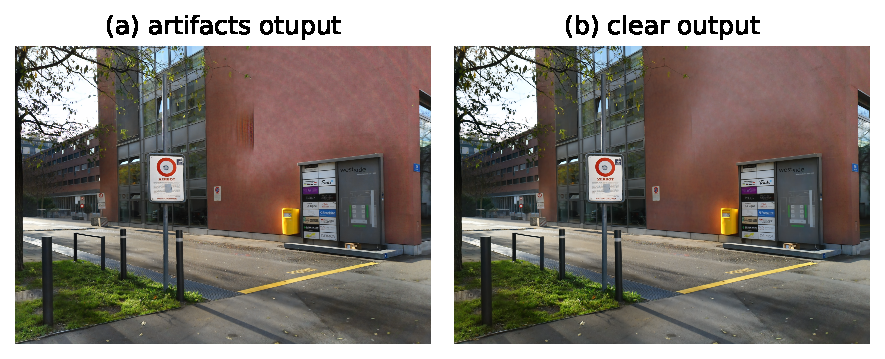
\includegraphics[width=\textwidth]{images/visualize_artifacts}
        \end{center}
    \end{minipage}

    \vspace{0.2em}
    \textbf{Visual Comparison of Reconstructed Images Trained Using Different Input Patch Sizes}
    \vspace{-0.8em}
    \begin{center}
        \includegraphics[width=0.455\textwidth]{images/results}
        \includegraphics[width=0.48\textwidth]{images/results2}
    \end{center}

    \begin{minipage}[t]{0.6\textwidth}
        \vspace{-1.4em}
        \textbf{Abalation Study on Using Different Ensemble Strategy During Testing} 
        \begin{center}
            \includegraphics[width=0.8\textwidth]{images/ablation}
        \end{center}
    \end{minipage}
    \hfill
    \begin{minipage}[t]{0.4\textwidth}
        \vspace{0.1em}
        \begin{center}
        \begin{minipage}{0.7\linewidth}
            \begin{center}
            \textbf{Scan the Qr-Code}: \\
            \vspace{0.5em}\textbf{Github} \& \textbf{Preprint} \& \textbf{Contact Us}
            \end{center}
        \end{minipage}
        \begin{minipage}{0.24\linewidth}
            \begin{center}
                \includegraphics[width=\linewidth]{images/qr-code}
            \end{center}
        \end{minipage}
        \end{center}
    \end{minipage}
}

%%%%%%%%%%%%%%%%%%%%%%%%%%%%%%%%%%%%%%%%%%%%%%%%%%%%%%%%%%%%%%%%%%%%%%%%%%%%%%
\headerbox{\bf\color{white} Method}{name=abstract,column=0,below=contribution,span=2}{
    \textbf{\color{red}Network Architecture:} The proposed HERN is a dual-path network, which consists of a global information path and a local information path.
    \begin{itemize}
        \item The global Information Path in green is based on RCAN but without attention unit. Besides, the autoencoder mechanism is used before the input features and after output features to enlarge the receptive field as well as reduce computational complexity.
        \item The Local Information Path in yellow is based on MSRN. It aims to extract local information such as textures and edges that destroyed in the encoder downsampling of the global information path.
        \item Further, a Pyramid Full-Image Encoder that extracts high-level characteristics in fix-resolution (192*192 px) is used to regularize local artifacts, which may be caused by resolution un-consistent.
    \end{itemize}
    \vspace{-0.5em}
    \begin{center}
     \includegraphics[width=0.8\textwidth]{images/RAW2RGBNet_architecture.pdf}
    \end{center}
    \vspace{-0.5em}
    \textbf{\color{red}Loss function:}
    \vspace{-0.5em} 
    \begin{equation}
        \mathcal{L}_1(\theta) = \frac{1}{N} \sum_{n=1}^{N} \left| \Phi (\rm{x}_i;\theta) - \rm{y}_i\right|,
        \vspace{-0.5em} 
    \end{equation}
    where $\Phi$ is the network function and $\theta$ represents the learnable parameters, $N$ is the batch size, and $\rm{x}_i$, $\rm{y}_i$ are the patch pairs of RAW image and RGB image.
}

\end{poster}
\end{document}
